%\include{begin}
\documentclass[a4j,titlepage]{jarticle}
\usepackage[dvipdfmx]{graphicx,epsfig}
\usepackage{longtable}
\usepackage{textcomp}
\usepackage{float}
\usepackage{ascmac}
\usepackage{fancybox}
\usepackage{url}


\begin{document}
\section{生活紹介}

\subsection{日時・場所}

\begin{tabular}{p{2zw}rp{38zw}}
  日時 & : & 2017年4月9日(日) 10:43 $\sim$ 11:25 \\ %09:20 $\sim$ 10:10 \\
  場所 & : & つどいの広間
\end{tabular}

\subsection{目的}
新入生の不安を解消する.

\subsection{イベント内容}
新入生の不安を解消するために以下の内容をパワーポイントを用いて紹介する.各紹介ごとにフリートークの時間を儲け,その紹介で疑問に感じたこと等を質問してもらう.また,各紹介では簡単なクイズを執り行う.

\begin{itemize}
\item 高知工科大学・情報学群について \\
  本大学の学内行事や情報学群で学べる内容について紹介する.
\item 一人暮らしについて \\
  一人暮らしをする際に注意する点や実際の経験を元に失敗談を紹介する.
\end{itemize}

各項目の持ち時間は15分である.またフリートークは8分とする.各項目ではクイズやインタビューを行う.クイズは挙手を行うだけの簡単なクイズとする.

\subsection{タイムスケジュール}
\begin{longtable}{p{3zw}p{39zw}}

%09:20
10:43 & \textbf{イベント開始} \\
      & \ \ \textbullet \ \ 司会がイベントの説明を行い,プレゼンターの紹介を行う \\
      & \ \ \textbullet \ \ プレゼンターは待機場所に待機しておく \\
%09:23
10:45 & \textbf{生活紹介 東} \\
%09:38
11:00 & \textbf{生活紹介 高橋(慎)} \\
%09:46
11:15 & \textbf{質問コーナー} \\
      & \ \ \textbullet \ \ 一人暮らしについて等の質問をスタッフが回答する. \\
      & \ \ \textbullet \ \ スクリーンには紹介した内容をまとめたスライドを表示しておく \\
%10:09
11:22 & \textbf{まとめ} \\
      & \ \ \textbullet \ \ 終了1分前に司会が全体の感想を述べた後に,これからトイレ休憩という趣旨を伝える \\
%10:10
11:25 & \textbf{イベント終了後} \\


\end{longtable}


\subsection{人員配置}
\begin{itemize}
\item 機器の操作 : 東,高橋(慎) \\
\item プレゼンター : 東,高橋(慎) \\
\end{itemize}

\subsection{全体配置}
\begin{figure}[h]
  \begin{center}
    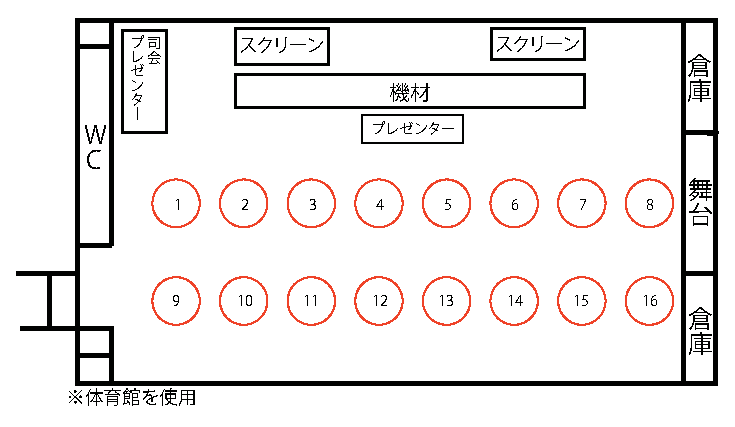
\includegraphics[scale=0.9]{./23/seikatsu.eps}
    \caption{体育館配置図}
    \label{fig:A1}
  \end{center}
\end{figure}

\subsection{必要物品}
 \begin{itemize}
 \item プロジェクター:1台
 \item スクリーン:1枚
 \item PC:1台
 \item マイク:3本
 \item 机:1個
 \item 椅子:1個
 \end{itemize}

\subsection{備考}
 \begin{itemize}
 \item プレゼンターは司会のマイクを使用する
 \item プレゼンターは紹介が終わった後自分の班に戻る
 \item 発表スライドの最後にまとめのスライドを作成し,フリートークの時に流す
 \item フリートークで話がとどこおるときは,スタッフから話を振る
 \end{itemize}

%\include{end}
\end{document}
